\chapter*{Dodatak: Prikaz aktivnosti grupe}
		\addcontentsline{toc}{chapter}{Dodatak: Prikaz aktivnosti grupe}
		
		\section*{Dnevnik sastajanja}
		
%		\textbf{\textit{Kontinuirano osvježavanje}}\\
%		
%		 \textit{U ovom dijelu potrebno je redovito osvježavati dnevnik sastajanja prema predlošku.}
		
		\begin{packed_enum}
			\item  sastanak
			
			\item[] \begin{packed_item}
				\item Datum: 18. listopada 2023.
				\item Prisustvovali: Vedran Ćutić, Antonio Glavaš, Marina Hrbud, Lara Marčec, Jakov Novak, Marko Varga, Nikola Vlahović
				\item Teme sastanka:
				\begin{packed_item}
					\item  upoznavanje
					\item  analiza zadatka
					\item  postavljanje GitHub-a
				\end{packed_item}
			\end{packed_item}
			
			\item  sastanak
			\item[] \begin{packed_item}
				\item Datum: 20. listopada 2023.
				\item Prisustvovali: Vedran Ćutić, Antonio Glavaš, Marina Hrbud, Lara Marčec, Jakov Novak, Marko Varga, Nikola Vlahović
				\item Teme sastanka:
				\begin{packed_item}
					\item  uvodni sastanak s asistentom i demonstratoricom 
					\item  razrješavanje upita o osnovnim funkcionalnostima aplikacije
					\item  dogovor oko alata i tehnologija
				\end{packed_item}
			\end{packed_item}
			
			\item  sastanak
			\item[] \begin{packed_item}
				\item Datum: 31. listopada 2023.
				\item Prisustvovali: Vedran Ćutić, Antonio Glavaš, Marina Hrbud, Lara Marčec, Jakov Novak, Marko Varga, Nikola Vlahović
				\item Teme sastanka:
				\begin{packed_item}
					\item  pregled odrađenih zadataka
					\item  dogovor o vizualnom izgledu aplikacije
					\item  raspodjela daljnjih poslova i dogovor internih rokova za iste
				\end{packed_item}
			\end{packed_item}
			
			\item  sastanak
			\item[] \begin{packed_item}
				\item Datum: 7. studenog 2023.
				\item Prisustvovali: Vedran Ćutić, Antonio Glavaš, Marina Hrbud, Lara Marčec, Jakov Novak, Marko Varga, Nikola Vlahović
				\item Teme sastanka:
				\begin{packed_item}
					\item  zajednička diskusija o dosad odrađenim zadacima
					\item  konkretna raspodjela daljnjih poslova i uloga
				\end{packed_item}
			\end{packed_item}


   			\item  sastanak
			\item[] \begin{packed_item}
				\item Datum: 15. studenog 2023.
				\item Prisustvovali: Vedran Ćutić, Antonio Glavaš, Marina Hrbud, Lara Marčec, Jakov Novak, Marko Varga, Nikola Vlahović
				\item Teme sastanka:
				\begin{packed_item}
					\item  pregled svih odrađenih zadataka
					\item  diskusija o predaji projekta 17.11.
     					\item  deployment aplikacije
				\end{packed_item}
			\end{packed_item}
			
			\item  sastanak
			\item[] \begin{packed_item}
				\item Datum: 11. prosinca 2023.
				\item Prisustvovali: Vedran Ćutić, Antonio Glavaš, Marina Hrbud, Lara Marčec, Jakov Novak, Marko Varga, Nikola Vlahović
				\item Teme sastanka:
				\begin{packed_item}
					\item  diskusija o ostvarenom uspjehu nakon prve predaje
					\item  detaljni pregled preostalih zadataka
					\item  raspodjela poslova
				\end{packed_item}
			\end{packed_item}

			\item  sastanak
			\item[] \begin{packed_item}
				\item Datum: 21. prosinca 2023.
				\item Prisustvovali: Jakov Novak, Marko Varga, Nikola Vlahović
				\item Teme sastanka:
				\begin{packed_item}
					\item  diskusija o daljnjem razvoju backenda aplikacije
					\item  detaljni pregled preostalih zahtjeva
          \item  diskusija o testovima (junit i Selenium)
					\item  raspodjela poslova
				\end{packed_item}
			\end{packed_item}
			
			\item  sastanak
			\item[] \begin{packed_item}
				\item Datum: 10. siječnja 2024.
				\item Prisustvovali: Vedran Ćutić, Antonio Glavaš, Marina Hrbud, Lara Marčec, Jakov Novak, Marko Varga, Nikola Vlahović
				\item Teme sastanka:
				\begin{packed_item}
					\item  pregled odrađenih zadataka
					\item  dogovor o daljnjem nastavku rada
				\end{packed_item}
			\end{packed_item}

			\item  sastanak
			\item[] \begin{packed_item}
						\item Datum: 12. siječnja 2024.
						\item Prisustvovali: Vedran Ćutić, Antonio Glavaš, Marina Hrbud, Lara Marčec, Marko Varga, Nikola Vlahović
						\item Teme sastanka:
						\begin{packed_item}
							\item  sastanak s demonstratoricom
							\item  dogovor o daljnjem nastavku rada
						\end{packed_item}
			\end{packed_item}

			\item  sastanak
			\item[] \begin{packed_item}
						\item Datum: 15. siječnja 2024.
						\item Prisustvovali: Vedran Ćutić, Antonio Glavaš, Marina Hrbud, Lara Marčec, Jakov Novak, Marko Varga, Nikola Vlahović
						\item Teme sastanka:
						\begin{packed_item}
							\item  pregled odrađenih zadataka
							\item  dogovor o daljnjem nastavku rada
							\item  krajnji dogovor za dokumentaciju i izradu prezentacije
						\end{packed_item}
			\end{packed_item}
			
			\item  sastanak
			\item[] \begin{packed_item}
						\item Datum: 17. siječnja 2024.
						\item Prisustvovali: Vedran Ćutić, Antonio Glavaš, Marina Hrbud, Lara Marčec, Jakov Novak, Marko Varga, Nikola Vlahović
						\item Teme sastanka:
						\begin{packed_item}
							\item  testiranje aplikacije
							\item  pregled frontenda
							\item  pregled backenda
							\item  krajnji dogovor za dokumentaciju i izradu prezentacije
							\item  dovogor za predaju projekta
						\end{packed_item}
			\end{packed_item}
			
			%
			
		\end{packed_enum}
		
		\eject
		\section*{Tablica aktivnosti}
		
			\textbf{\textit{Kontinuirano osvježavanje}}\\
			
			 \textit{Napomena: Doprinose u aktivnostima treba navesti u satima po članovima grupe po aktivnosti.}

			\begin{longtblr}[
					label=none,
				]{
					vlines,hlines,
					width = \textwidth,
					colspec={X[7, l]X[1, c]X[1, c]X[1, c]X[1, c]X[1, c]X[1, c]X[1, c]}, 
					vline{1} = {1}{text=\clap{}},
					hline{1} = {1}{text=\clap{}},
					rowhead = 1,
				} 
			

				\SetCell[c=1]{c}{} & \SetCell[c=1]{c}{\rotatebox{90}{\textbf{Vedran Ćutić }}} & \SetCell[c=1]{c}{\rotatebox{90}{\textbf{Antonio Glavaš }}} &	\SetCell[c=1]{c}{\rotatebox{90}{\textbf{Marina Hrbud }}} & \SetCell[c=1]{c}{\rotatebox{90}{\textbf{Lara Marčec }}} &	\SetCell[c=1]{c}{\rotatebox{90}{\textbf{Jakov Novak }}} & \SetCell[c=1]{c}{\rotatebox{90}{\textbf{Marko Varga }}} &	\SetCell[c=1]{c}{\rotatebox{90}{\textbf{Nikola Vlahović }}} \\  

				Upravljanje projektom 		& 11 & 11 & 11 & 11 & 11 & 11 & 11\\
				Opis projektnog zadatka 	&  &  & 2 &  &  & 2 & \\ 
				
				Funkcionalni zahtjevi       &  &  &  & 1 &  &  & 2\\
				Opis pojedinih obrazaca 	&  &  &  & 2 &  &  & 1\\ 
				Dijagram obrazaca 			&  &  &  &  & 2 & 1 &  \\ 
				Sekvencijski dijagrami 		&  &  &  & 4 &  &  &  \\ 
				Opis ostalih zahtjeva 		&  &  &  & 1 &  &  &  \\ 

				Arhitektura i dizajn sustava	 &  & 3 &  &  &  &  &  \\ 
				Baza podataka				& 2 &  & 4 &  &  & 2 &   \\
				Dijagram razreda 			&  & 3 &  &  &  &  &   \\ 
				Dijagram stanja				&  &  & 2 &  &  &  &  \\ 
				Dijagram aktivnosti 		&  &  &  & 2  &  &  &  \\ 
				Dijagram komponenti			& 3 &  &  &  &  &  &  \\
				Korištene tehnologije i alati 		  &  &  & 1  &  &  &  \\
				Ispitivanje programskog rješenja 	  & 2 &  &  &  &  & & 13 \\
				Dijagram razmještaja			&  & 3 &  &  &  &  &  \\
				Upute za puštanje u pogon 		&  &  &  &  & 1 & 1 &  \\  
				Dnevnik sastajanja 			& 1 &  & 1 & 2 &  & 1 &  \\
				Zaključak i budući rad 		&  &  & 2 &  &  &  &  \\  
				Popis literature 			&  &  &  &  &  &  &  \\  
				&  &  &  &  &  &  &  \\ \hline 
				\text{izrada front-end stranice} 			&  &  & 20 & 30 & 15 & 15 &  \\  
				\text{izrada baze podataka} 		 	&  &  & 4 &  & 1 & 4 & \\
				\text{spajanje s bazom podataka} 		& 1 &  &  &  & 6 & 3 &  \\
		        \text{back-end}	& 14 & 15 &  &  & 35 & 20 & 25\\
		        \text{deployment}          				&  &  &  &  &  10 & 6 &\\ 
			\end{longtblr}
					
					
		\eject
		\section*{Dijagrami pregleda promjena}

%		\textbf{\textit{dio 2. revizije}}\\
%		\textit{Prenijeti dijagram pregleda promjena nad datotekama projekta. Potrebno je na kraju projekta generirane grafove s gitlaba prenijeti u ovo poglavlje dokumentacije. Dijagrami za vlastiti projekt se mogu preuzeti s gitlab.com stranice, u izborniku Repository, pritiskom na stavku Contributors.}

		\begin{figure}[H]
			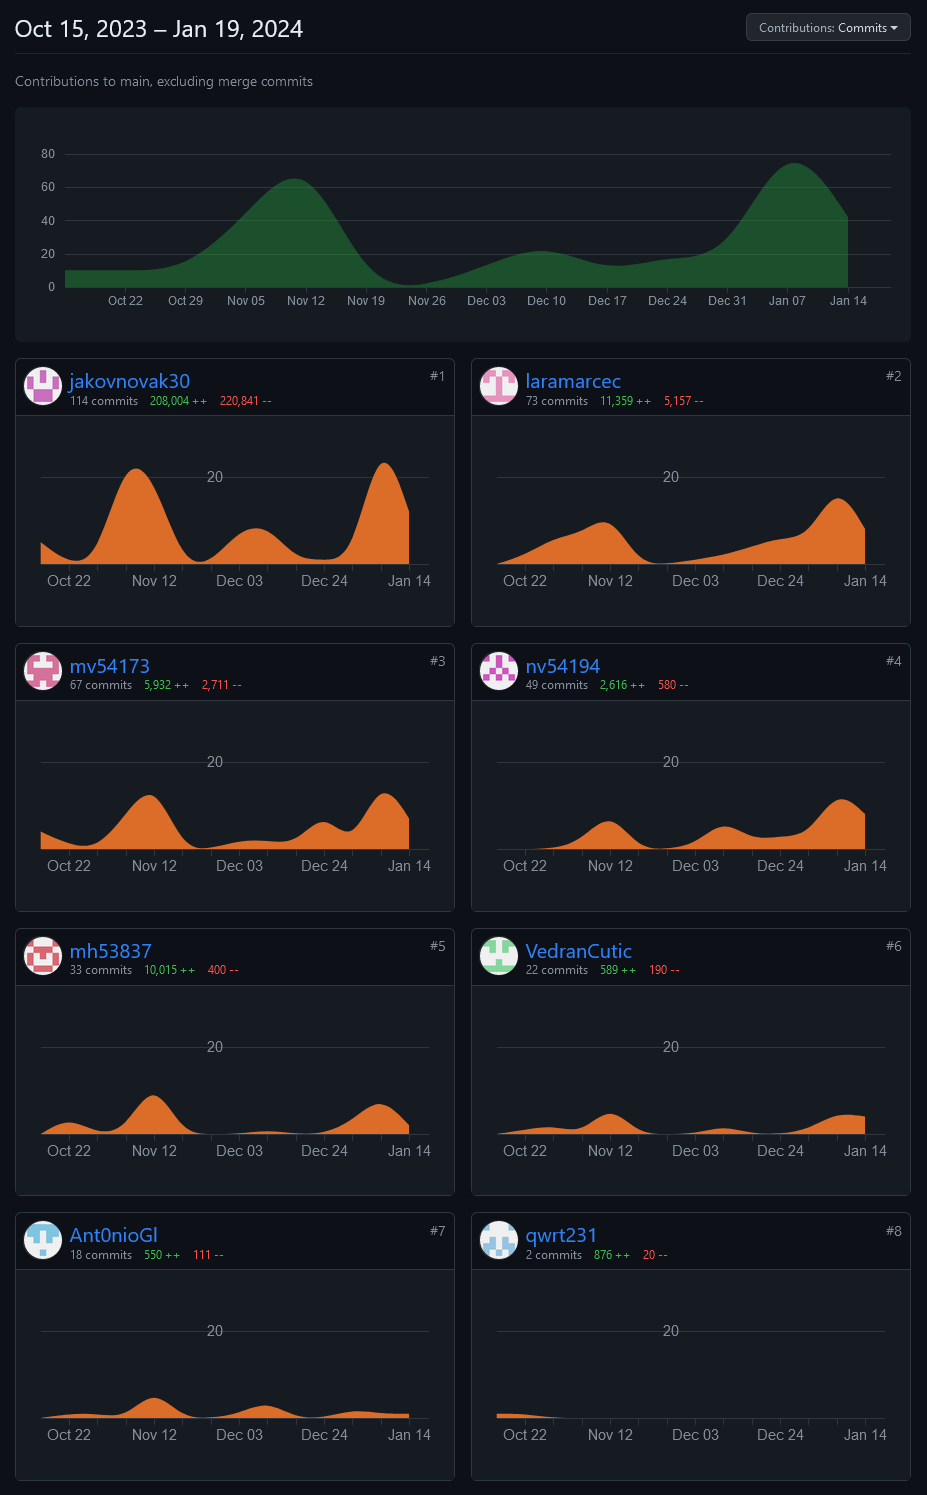
\includegraphics[scale=0.53]{slike/pregled_promjena.png}
			\centering
			\caption{Dijagrami pregleda promjena}
			\label{fig:pregled_promjena}
		\end{figure}
	
